\section{Evaluation}

\begin{figure}
\centering
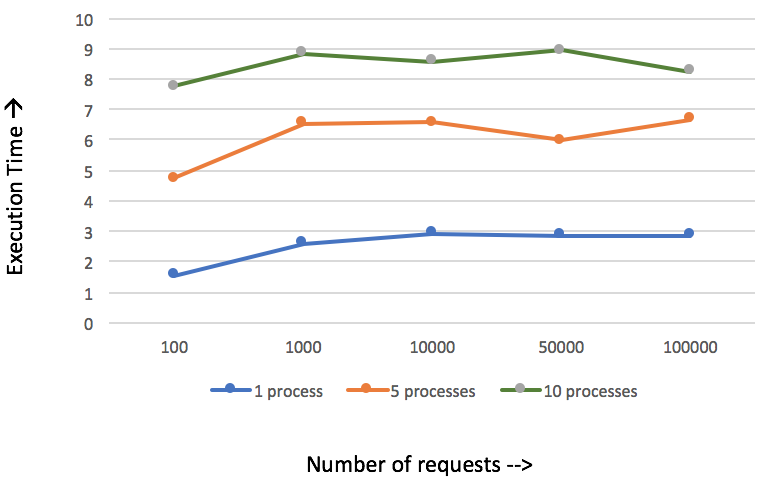
\includegraphics[height=2in, width=3.2in]{images/F-HC-SF-R.png}
\caption{Execution time (in ms) of increasing number of READ requests generated from each process running in 5 clients. These requests perform action on the same file.}~\label{fig:figure3}
\end{figure}

In this section, we present our results for the different experiments performed by varying contention and workload types.

\subsection{Single client}

In the first set of experiments, we wanted to measure the time taken for one single read and write request and benchmark it against the round trip time(RTT) for a simple ICMP message. The first request issued from any client process is directed to a random server chosen from the list of servers in the Raft cluster. Hence, it may either directly reach the leader or reach a follower and get re-directed to the leader. We observed that a single read request took 3-5ms if the request reached the leader directly, and  4-11ms on a miss, while a single write request took 2-4ms on hitting the leader and 3-10ms otherwise. Because there was a huge range in the results obtained for a single request, it was only natural to evaluate the total time taken for a thousand requests to obtain the average for a single request. Fig.\ref{fig:figure2} gives the average read and write time while running increasing number of processes in one client and 1000 requests in each of these processes. While a single read took more time than a single write, we observe that the average read time is consistently lesser than the write time. While, read calls a majority of other servers to ensure it is still the leader, a write call does extra work of appending the log entry on a majority of other servers. Hence, a write call taking more time than read is as expected considering the algorithm design. Also, with the increase in number of processes, the average read and write time increase almost linearly. The important point to note here is that the ICMP RTT is 0.587 and hence, the difference of 1.1ms for a read and 1.9ms for a write is the overhead Raft takes for its protocol execution. 

\subsection{Multiple clients}

In the second set of experiments, we measured the affect of issuing a large set of sequential requests on Raft. For this, we issued sequential requests ranging from 100-100000 using five clients. Six experiments were performed by changing the number of concurrent requests to 5, 25 and 50(1, 5 and 10 processes in each client), for a workload of 100\% read and 100\% write.

Fig. \ref{fig:figure3} shows the result for running increasing number of sequential results on Raft using 5, 25 and 50 concurrent requests for a workload of 100\% reads, while Fig. \ref{fig:figure4} shows the same for 100\% write requests. Both the graphs show a very similar pattern, except that average write time at every point is greater than the average read time for the same number of requests and processes. The graphs also clearly show more the number of concurrent requests, higher is the average read and write time taken. However, increase in the number of sequential requests has no effect on the execution time for both reads and writes. Hence, Raft is robust under low concurrency and high request bombardment.
This naturally brought us to the next set of experiments which dealt with increase in concurrent requests to Raft, while keeping the sequential requests consistent.

\begin{figure}
\centering
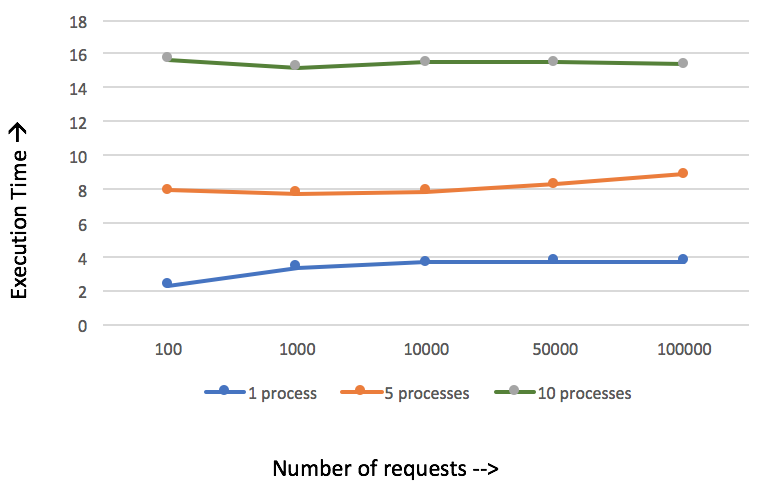
\includegraphics[height=2in, width=3.2in]{images/F-HC-SF-W.png}
\caption{Execution time (in ms) of increasing number of WRITE requests generated from each process running in 5 clients. These requests perform action on the same file.}~\label{fig:figure4}
\end{figure}

\begin{figure}
\centering
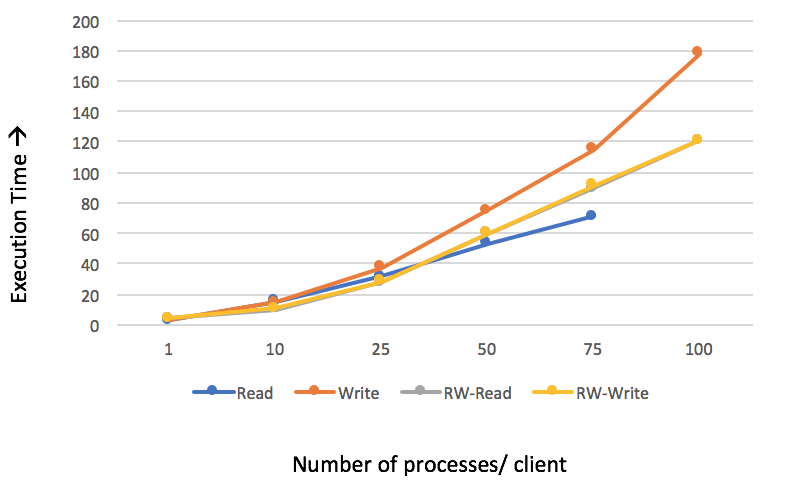
\includegraphics[height=2in, width=3.2in]{images/F-VHC-SF.png}
\caption{Execution time (in ms) of 1000 READ and WRITE requests generated from each process running in 4 clients. These requests perform action on the same file.}~\label{fig:figure5}
\end{figure}

In the next phase, we used 4 clients and increased the number of processes running in each client so as to load Raft with higher number of concurrent requests. Fig.\ref{fig:figure5} displays the result for running 1000 requests in each process and increasing the number of processes from 1 to 100 in each client. In this and all previous experiments, all actions of read and write were done on the same file. However, we also wanted to judge the performance when the actions were performed on different files, to eliminate extra concurrency overhead associated with potential file locks. Both graphs show worse than linear and better than exponential increase in the time. We did not go beyond 100 processes per client to avoid overloading the clients. In future, we would like to add more clients to increase concurrency even further and observe whether the time increase is more linear or exponential. However, it is certain that Raft gets overloaded with 400 concurrent requests, which was also noticed in more frequent leader election process. This election frequency was increased, as the latency for appendEntries requests increased, resulting in further overloading the Raft system. 

The graphs also show the execution time for a workload of 50\% reads and 50\% writes. The average timings for the reads and writes are separately plotted on the graph. While we expected that this workload would lead to a line in between 100\% reads and 100\% writes, we however, assumed that the reads in 50-50 workload would take lesser time than writes, as observed before. However, it was seen that in such a workload, both reads and writes took very similar time, and hence the line for RW-read is hidden by RW-write in the graphs. This shows that in such a workload, writes block the reads and both end up taking similar but lesser time than a workload full of writes. 

The third observation was in terms of action performed on same and different files, as shown in the two graphs respectively. While timings were almost similar in the two graphs until 75 processes, the writes took 20\% more time while performed on the same file for 100 processes. While operations on same file is expected to take longer than for different file, without extended results, we would not be able to make a conclusive comparison pattern for the same. 


\begin{figure}
\centering
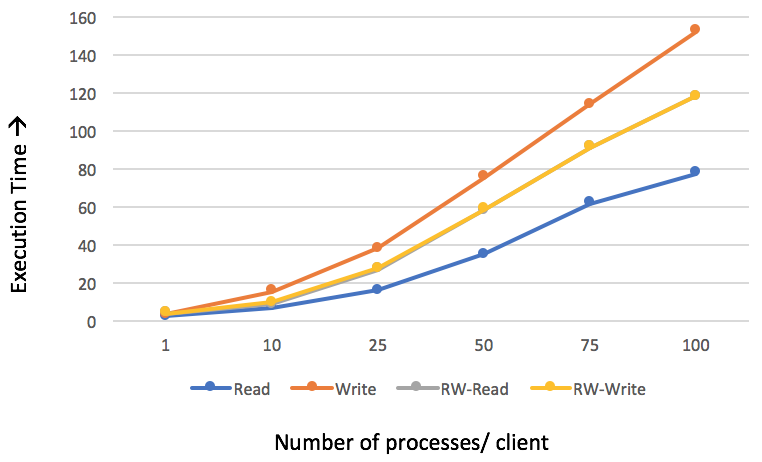
\includegraphics[height=2in, width=3.2in]{images/F-VHC-DF.png}
\caption{Execution time (in ms) of 1000 READ and WRITE requests generated from each process running in 4 clients. These requests perform action on different files.}~\label{fig:figure6}
\end{figure}










